\label{Hardwareimpl}

Nach erfolgreichem Drucken des Gehäuses, wurde das Arduino Modul mithilfe on Schrauben an die dafür vorgesehene Stelle befestigt, das PIN-Breadboard verklebt und der Sensor außerhalb des Gehäuses montiert. Das \ac{LCD}-Display, die \ac{LED}s und die Taster wurden anschließend, wie in Abbildung \ref{fig:Deckel} zu sehen ist, auf dem Deckel befestigt.

\begin{figure}[!hbt]
	\centering
	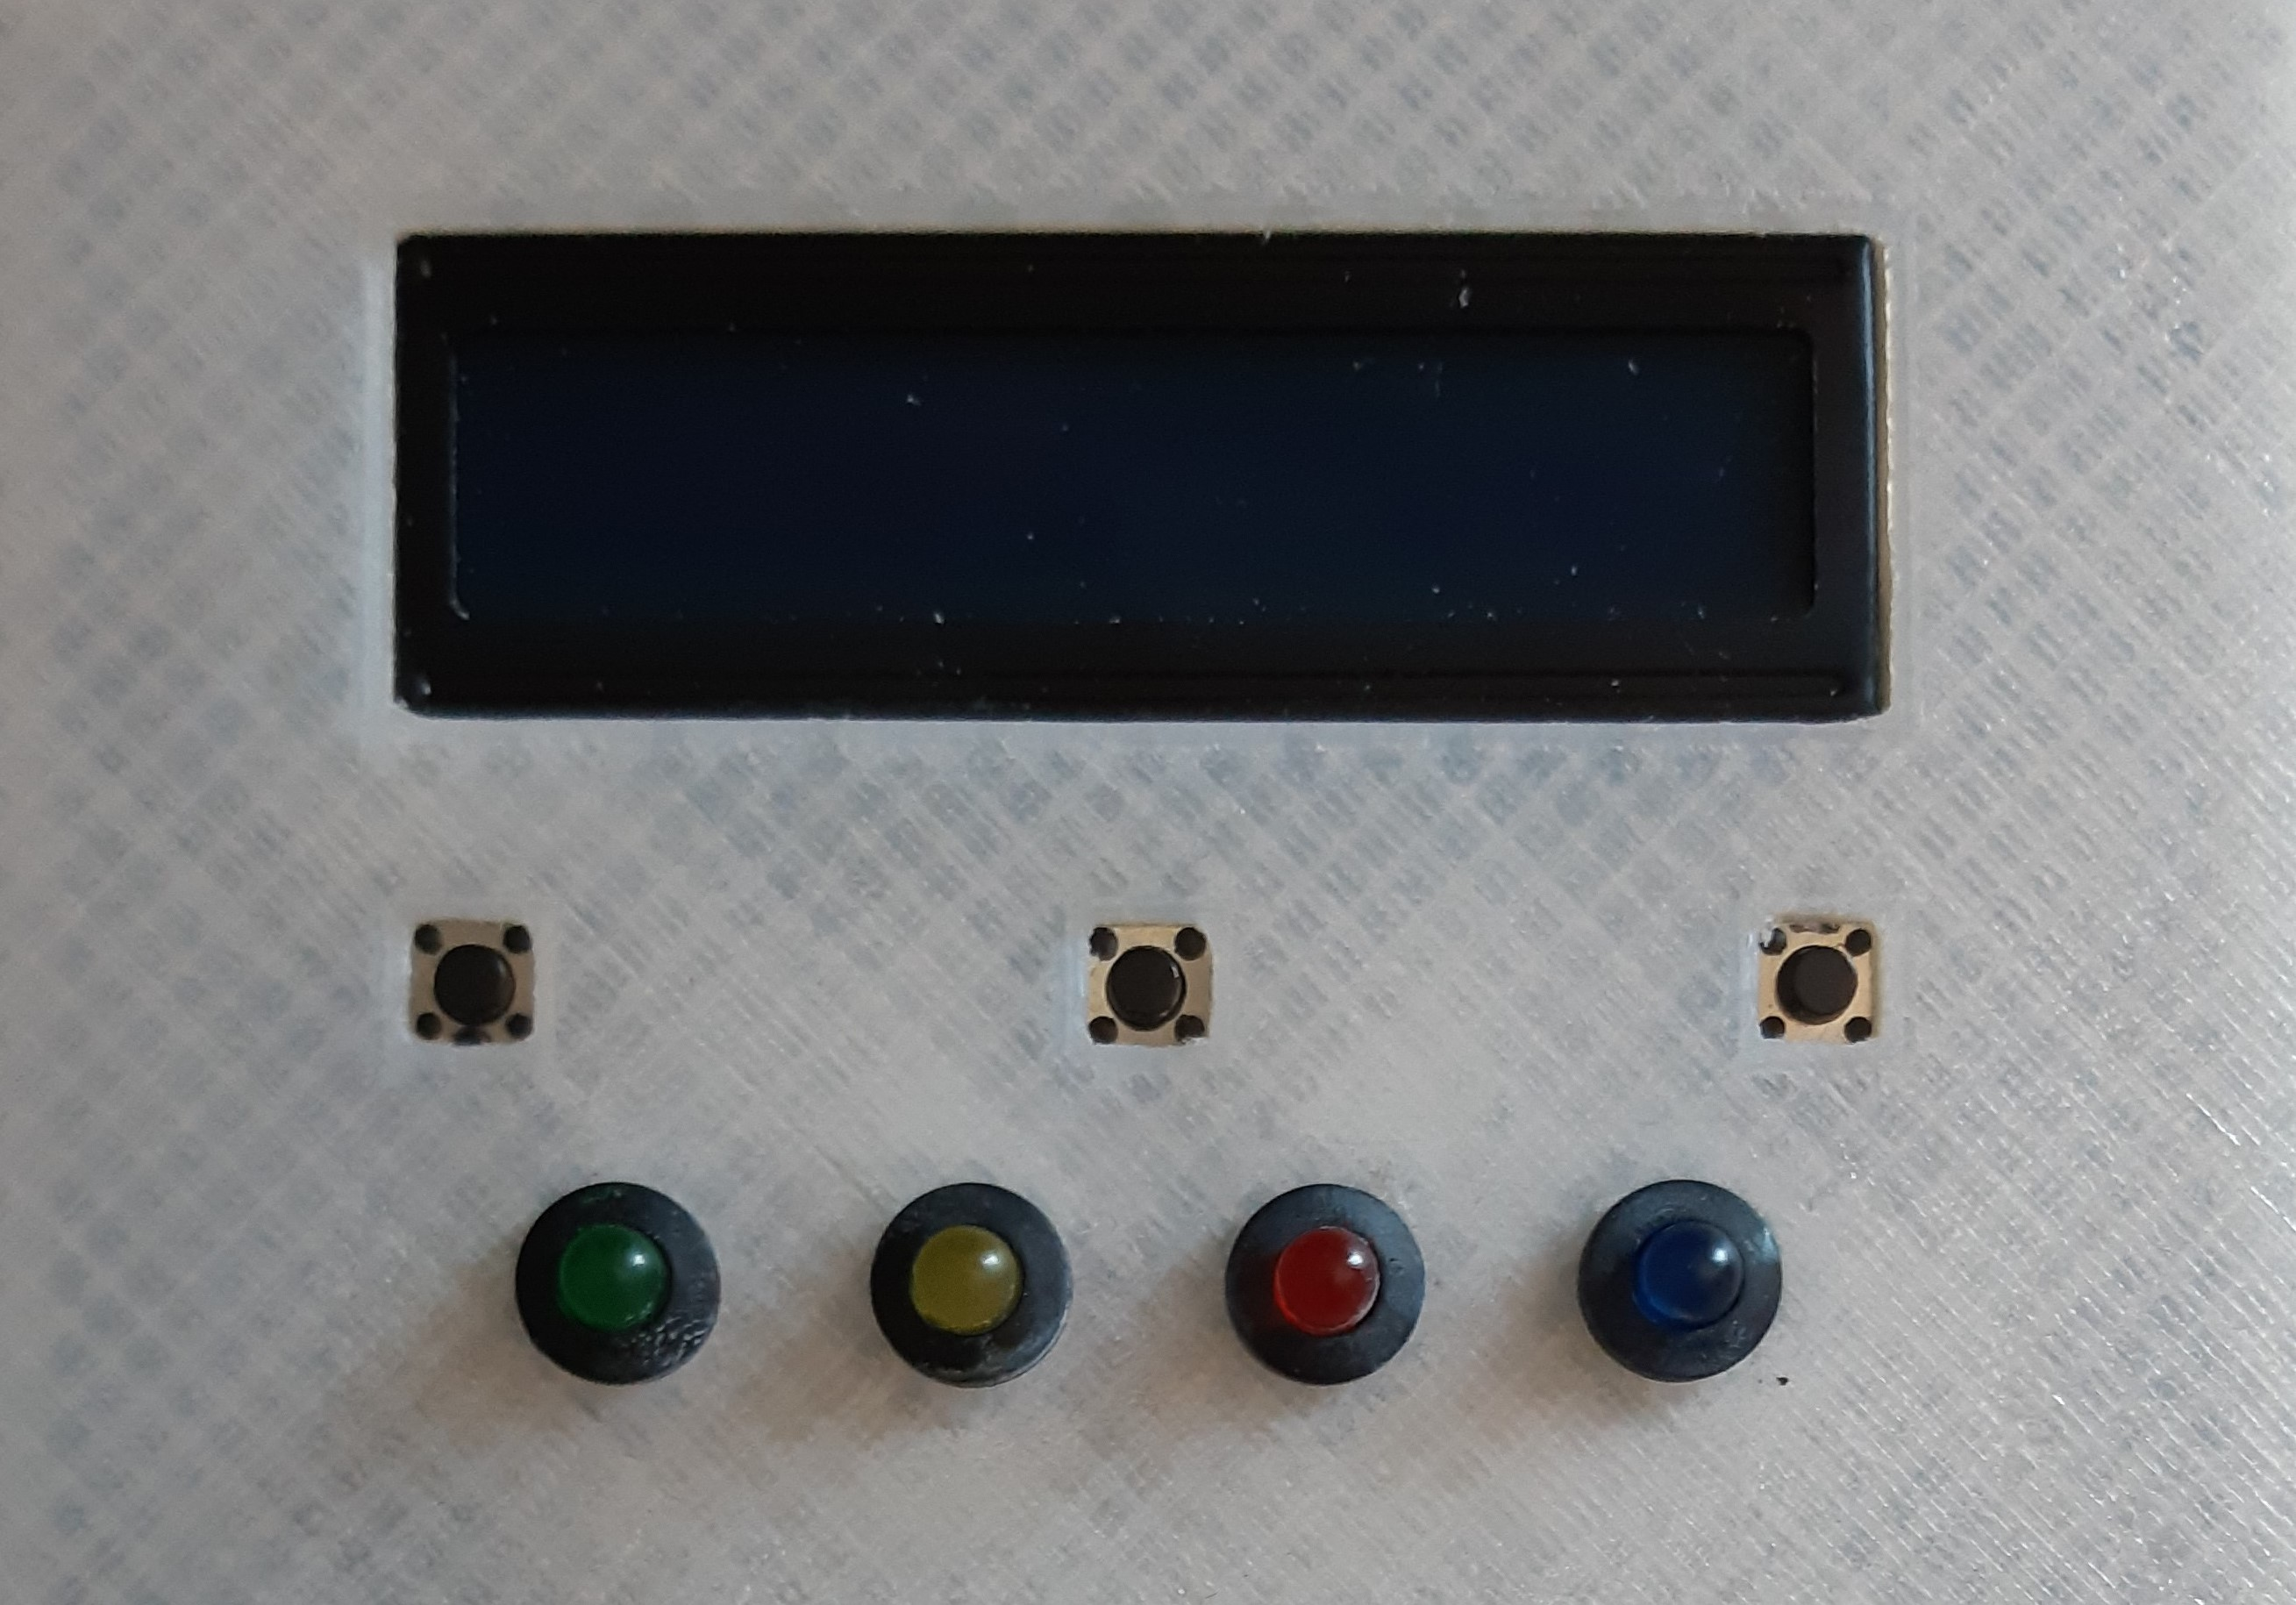
\includegraphics[width=0.3\linewidth]{Images/Deckel}
	\footnotesize \\Quelle: eigene Aufnahme
	\caption{3D-gedruckter Deckel des Gehäuses}
	\label{fig:Deckel}
\end{figure}

Die Entscheidung, das PIN-Breadboard für die Implementierung, wie in Abbildung \ref{fig:Einbau_AuB}, zu nutzen, hat den Vorteil mit sich gebracht, dass ohne großen Lötaufwand, die mitgelieferten Kabel aus dem Arduino-Kit nach Schaltplan verlegt werden konnten. Somit war die Kabelführung einfacher zu gestalten.

\begin{figure}[!hbt]
	\centering
	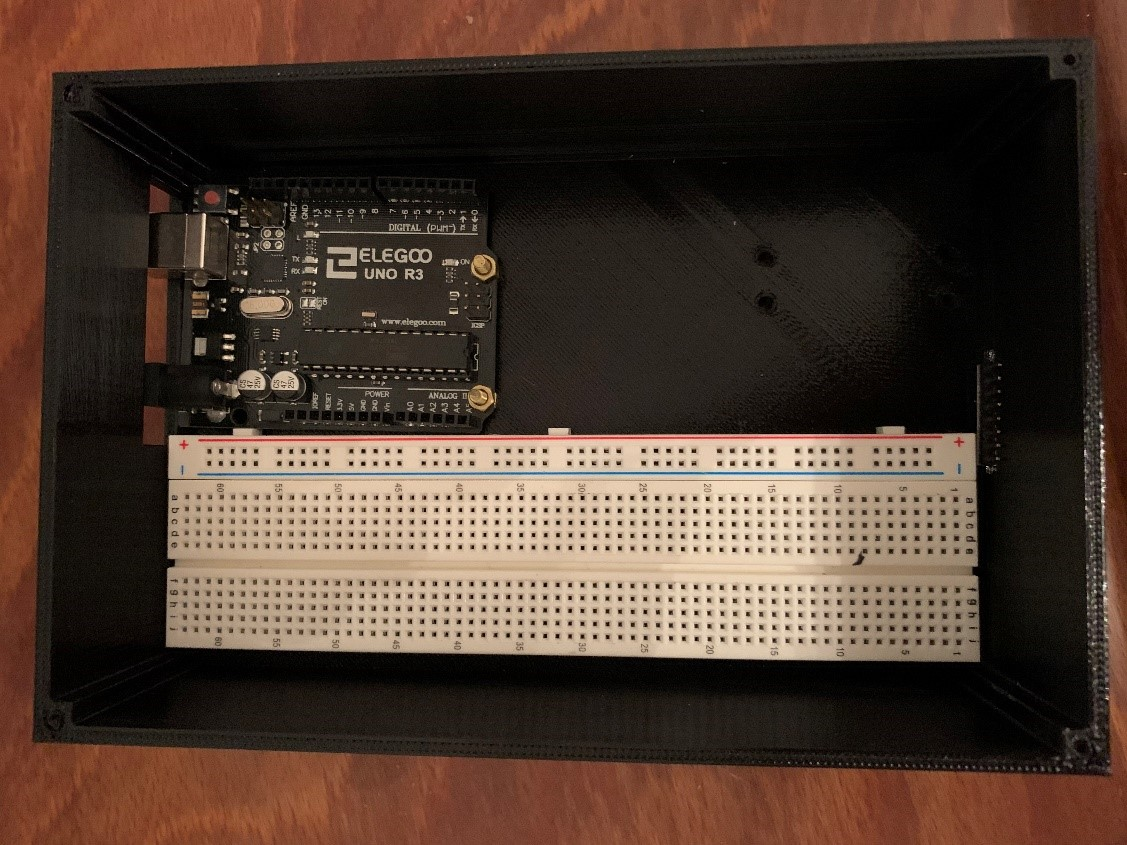
\includegraphics[width=0.3\linewidth]{Images/Einbau_AuB}
	\footnotesize \\Quelle: eigene Aufnahme
	\caption{Einbau des Arduinos und des PIN-Breadboards in der 3D-gedruckten Schale des Gehäuses}
	\label{fig:Einbau_AuB}
\end{figure}